\documentclass{article}
\usepackage{graphicx}
\usepackage{lipsum}
\usepackage[T2A]{fontenc}
\usepackage[utf8]{inputenc}

\graphicspath{ {./Results/} }

% \title{Quick Sort}
% \author{Dadmo}
% \date{\today}

\begin{document}
% \maketitle
\begin{titlepage}
    \begin{center}
    $\newline$
    \vspace{3.3cm}
    
    {\LARGE\textbf{Лабораторна робота №8\\"Piramide Sort"}}
    \vspace{10cm}
    \begin{flushright}
        \textbf{Роботу виконав:}\\Климентьєв Максим \\3-го курсу\\групи ФІ-21
    \end{flushright}
    \end{center}
\end{titlepage}
\newpage

\tableofcontents 
\section{Вбудована бібліотека Python}
\textbf{Heapq} --- Вбудована бібліотека Python, в якій реалізована черга з пріоритетами. Реалізація черги з пріоритетами виглядає як пірамідальне представлення (Купа) --- також відбуваються просіювання вгору та вниз. Відмінність полягає у меншій кулькості функцій. Присутнє лише перероблення списку на чергу з приорітетами, пуш в чергу, вилучення з черги, пуш та вилучення одночасно, пошук максимальних та мінімальних елементів, а також злиття списків.
\section{Piramide Sort}
\textbf{PiramideSort} --- клас, в якому максимально примітивно реалiзовано алгоритм сортування.
\newline
Надалі "дерево" --- масив, який цей клас використовує замість дерева.
Примітивність полягає у тому, що виконується сортування поелементно. Вилучається один елемент з "дерева", "перебудовується" "дерево" і так доти, доки не закінчаться елементи.
\newline

\section{Piramide Sort Test}
\textbf{Перевіряє чи масив відсортований завдяки певній варіації алгоритму чи ні.}

\section{Random Lists}
\textbf{RandomLists} --- клас, який має реалiзованi 6 варiантів генерацiї спискiв.
\begin{enumerate}
    \item \textbf{Повнiстю вiдсортований (sorted)} --- на вхід подається лише розмiр списку.
    \item \textbf{Випадковi (random)} --- на вхід подається лише розмiр списку.
    \item \textbf{Майже вiдсортований (almostsorted)} --- на вхід подається розмiр списку, та відсоток безпорядку.
    \item \textbf{Вiдсортованi в зворотному порядку (reverse)} --- на вхід подається лише розмiр списку.
    \item \textbf{Лише з декiлькома рiзними значеннями (somenumbers)} --- на вхід подається розмiр списку, та діапазон значень (Початок, Кiнець).
    \item \textbf{"Трикутнi" (triangular)} (перша половина є строго висхiдною послiдовнiстю, а друга половина є дзеркальним вiдображенням першої).
\end{enumerate}
\newpage

\section{Comparisions and Results}
% SORTED
    \subsection{Результати:}
    \textbf{Час виконання:}
    \newline
        % [scale=0.5]
        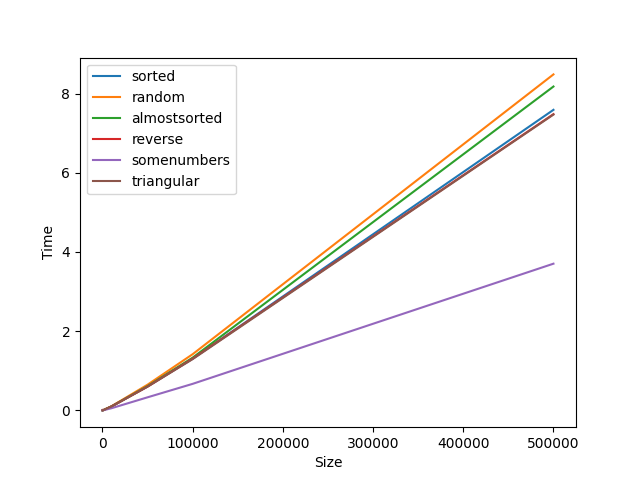
\includegraphics{triangular_Time_7_numbers.png}
    \subsection{Висновки:}
    \begin{enumerate}
        \item Лише з декiлькома рiзними значеннями сортуються швидше за усі інші види.
    \end{enumerate}
    \newpage

\end{document}